%----------------------------------------------------------------------------------------
%	CONSTANTS
%----------------------------------------------------------------------------------------

\newcommand{\hmwkTitle}{Report\ \#3}					% Assignment title
\newcommand{\hmwkClass}{Communication Networks}			% Course name
\newcommand{\hmwkClassTime}{}							% Workshop time
\newcommand{\hmwkClassInstructor}{}						% Tutor name
\newcommand{\hmwkAuthorName}{Ang LEE}					% Student name

\newcommand{\hmwkGraphicsPath}{img/}					% Graphics path
\newcommand{\hmwkCodePath}{code/}						% Code path

%----------------------------------------------------------------------------------------
%	TEMPLATE
%----------------------------------------------------------------------------------------

\documentclass{article}

\usepackage{fancyhdr}	% Required for custom headers
\usepackage{lastpage}	% Required to determine the last page for the footer
\usepackage{extramarks} % Required for headers and footers
\usepackage{graphicx}	% Required to insert images
\graphicspath{\hmwkGraphicsPath}
\usepackage{lipsum} 	% Used for inserting dummy 'Lorem ipsum' text into the template

\usepackage{float}
\usepackage{epstopdf}	% Required to insert .eps images
\usepackage{amssymb}
\usepackage{amsmath}
\usepackage[hidelinks]{hyperref}

% Python syntax highlighting
\usepackage{color}		% Required to define colors
\definecolor{commentColor}{RGB}{153,153,153}
\definecolor{stringColor}{RGB}{37,170,33}
\usepackage{listings}
\lstset{
	inputpath=\hmwkCodePath,
	language=Python,
	basicstyle=\footnotesize\ttfamily,
	keywordstyle=\color{blue},
	stringstyle=\color{stringColor},
	commentstyle=\usefont{T1}{pcr}{m}{n}\color{commentColor},
	breaklines=true,
	showstringspaces=false
}

% change \textbf textbf
\definecolor{bfcolor}{RGB}{221,75,57}
\DeclareTextFontCommand{\textbf}{\bfseries\color{bfcolor}}

% change \texttt color
\definecolor{ttcolor}{RGB}{0,103,179}
\DeclareTextFontCommand{\texttt}{\ttfamily\color{ttcolor}}

% change headings color
\usepackage{sectsty}
\definecolor{sectioncolor}{RGB}{0,102,33}
\sectionfont{\color{sectioncolor}}
\definecolor{subsectioncolor}{RGB}{26,131,171}
\subsectionfont{\color{subsectioncolor}}
\definecolor{subsubsectioncolor}{RGB}{0,51,102}
\subsubsectionfont{\color{subsubsectioncolor}}

% Margins
\topmargin=-0.45in
\evensidemargin=0in
\oddsidemargin=0in
\textwidth=6.5in
\textheight=9.0in
\headsep=0.25in

\linespread{1.1}		% Line spacing

% Set up the header and footer
\pagestyle{fancy}
\lhead{\hmwkTitle} % Header Left 
\chead{\hmwkAuthorName} % Header Center
\rhead{\hmwkClass} % Header Right
\lfoot{\url{https://github.com/leeang/Communication-Networks}} % Footer Left
\cfoot{} % Footer Center
\rfoot{Page\ \thepage\ of\ \pageref{LastPage}} % Footer Right
\renewcommand\headrulewidth{0.4pt} % Size of the header rule
\renewcommand\footrulewidth{0.4pt} % Size of the footer rule

\setlength\parindent{0pt} % Removes all indentation from paragraphs

%----------------------------------------------------------------------------------------
%	Problem and Section
%----------------------------------------------------------------------------------------

\newenvironment{homeworkProblem}[1]{
	\section*{#1}
	}{
}
\newenvironment{homeworkSection}[1]{
	\subsection*{#1}
	}{
}
\newcommand{\problemAnswer}[1]{
	\noindent\framebox[\columnwidth][c]{
		\begin{minipage}{0.98\columnwidth}
			#1
		\end{minipage}
	}
}

%----------------------------------------------------------------------------------------
%	Document
%----------------------------------------------------------------------------------------

\begin{document}

\newpage

%----------------------------------------------------------------------------------------
%	Section 1
%----------------------------------------------------------------------------------------

\begin{homeworkProblem}{Question 1.1}
Write the formulas for the average time spent by a customer in the system and the system occupancy of an M/M/1 queue.\\

The average time spent by a customer in the system:
\begin{equation}
T = \frac{\bar{N}}{\lambda} = \frac{1}{\mu-\lambda}
\end{equation}
where $\mu$ is the service rate and $\lambda$ is the arrival rate.
\end{homeworkProblem}

%--------------------------------------------

\begin{homeworkProblem}{Question 1.2}
What is the relationship between total time spent in the system, queueing delay, and service time? Similarly, what is the difference between the number of customers (packets) in the queue, that are currently serviced, and the total system occupancy?\\

\begin{equation}
T = \bar{x} + W
\end{equation}
Total time: $T$\\
Queuing delay (waiting time): $W$\\
Service time: $\bar{x}$
\end{homeworkProblem}

%--------------------------------------------

\begin{homeworkProblem}{Question 1.3}
Estimate the expected system size and the expected time spent in system based on your simulations. Then, compute the expected theoretical values (in Python or Matlab) for these.\\

\begin{equation}
T = \frac{1}{\mu-\lambda} = \frac{1}{4-3} = 1
\end{equation}
\begin{equation}
p = \frac{\lambda}{\mu} = \frac{3}{4}
\end{equation}
\begin{equation}
N = \frac{p}{1-p} = 3
\end{equation}

Mean theoretical delay: 1.000000\\
Mean theoretical size : 3.000000
\end{homeworkProblem}

%--------------------------------------------

\begin{homeworkProblem}{Question 1.4}
Compare the simulation results with theoretical values. For what number of arrivals do these two become similar (answer in terms of order of magnitude)?\\

Mean practical delay: 0.990398\\
Mean practical size : 2.982140\\

When the number of arrivals reaches \textbf{$10^5$}, the theoretical and empirical values become similar.

\begin{figure}[H]
\begin{minipage}[t]{0.5\linewidth}
\centering
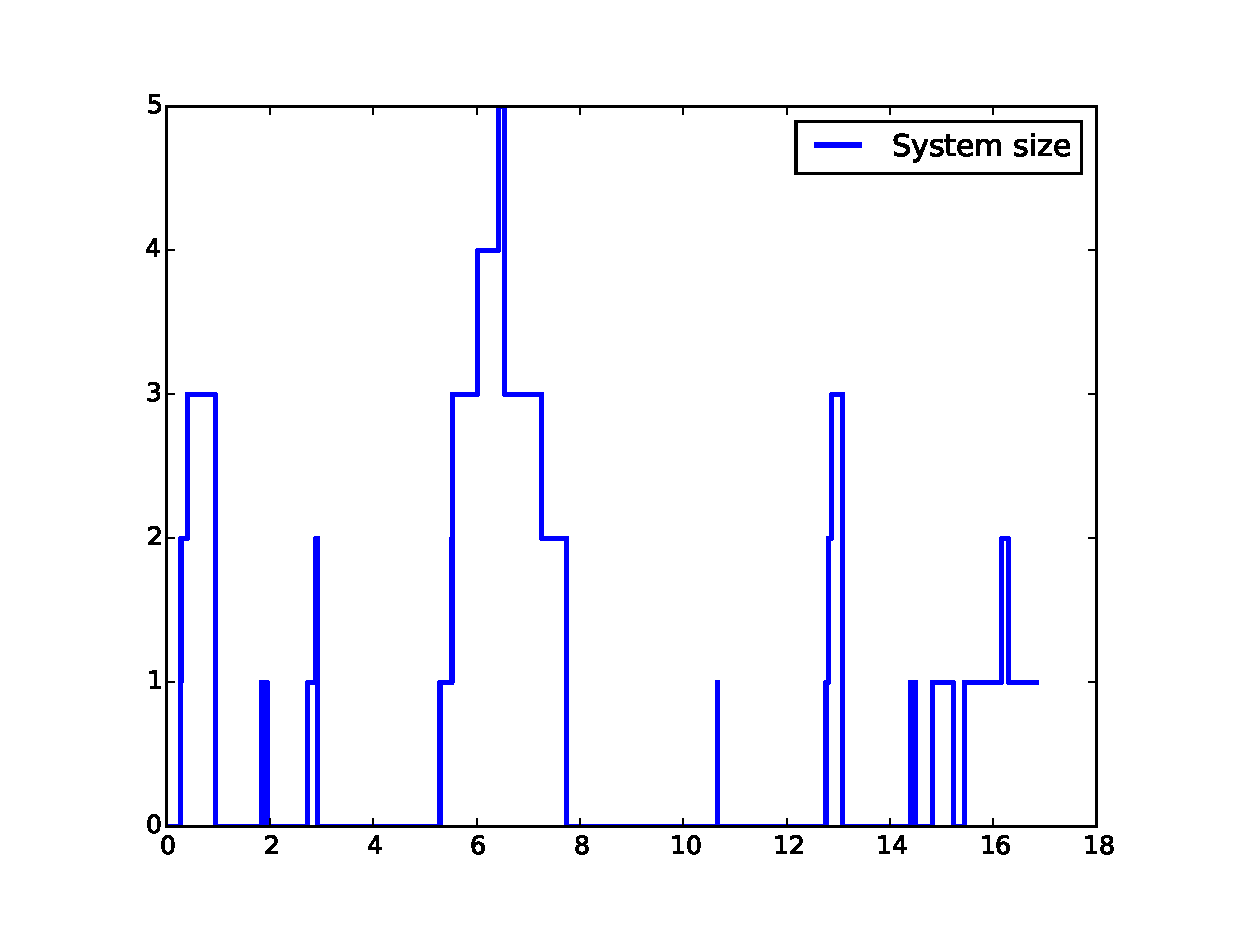
\includegraphics[width=3.3in]{mm1-system-size}
\caption{M/M/1 System Size}
\label{mm1-system-size}
\end{minipage}
\begin{minipage}[t]{0.5\linewidth}
\centering
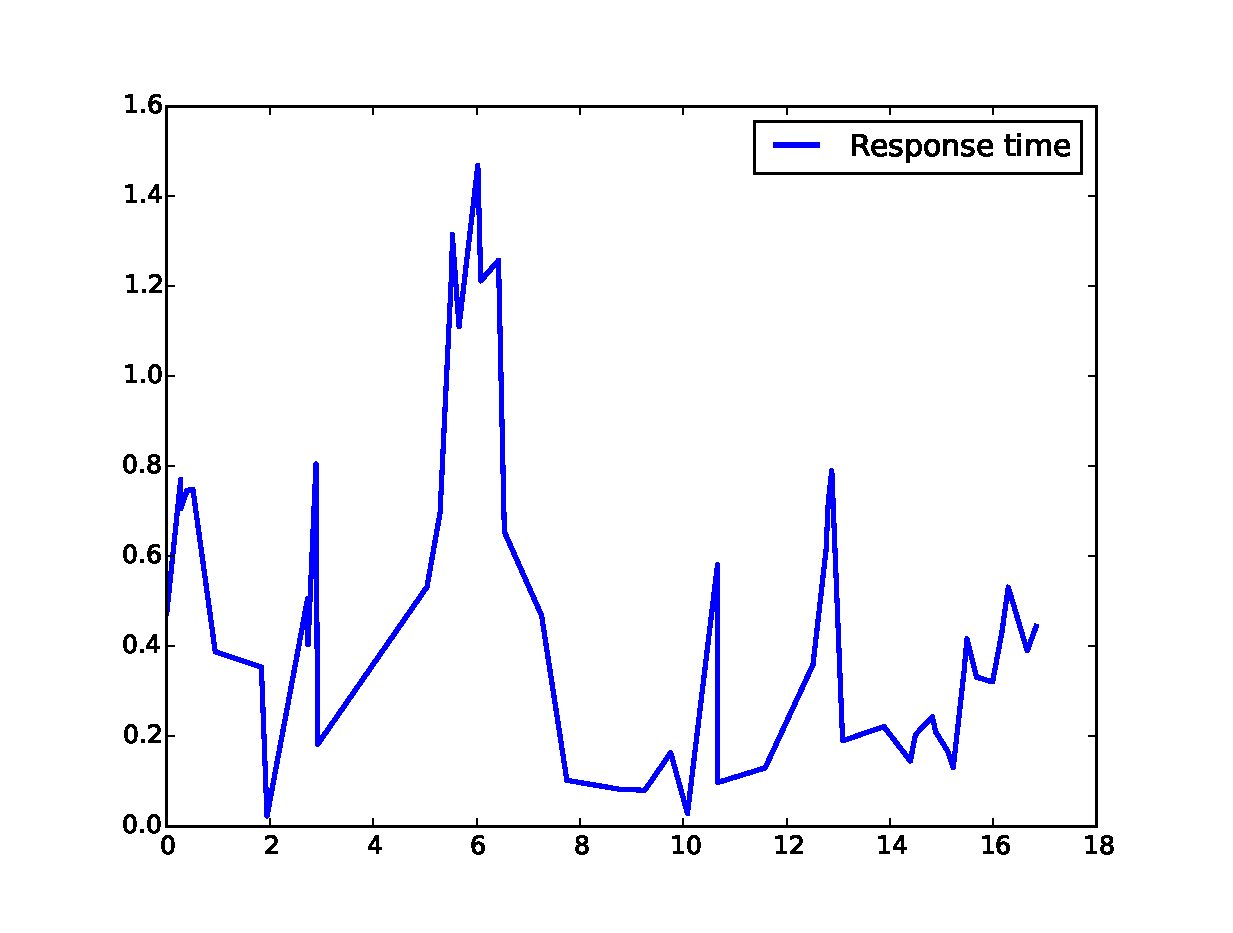
\includegraphics[width=3.3in]{mm1-response-time}
\caption{M/M/1 Response Time}
\label{mm1-response-time}
\end{minipage}
\end{figure}

\end{homeworkProblem}

%--------------------------------------------

\begin{homeworkProblem}{Question 1.5}
Experiment with other types of interarrival and service time combinations, e.g. M/D/1, D/M/1, D/D/1. You only need to provide practical calculation values.

%--------------------------------------------

\begin{homeworkSection}{M/D/1}

Mean practical delay: 0.639085\\
Mean practical size : 1.936220

\begin{figure}[H]
\begin{minipage}[t]{0.5\linewidth}
\centering
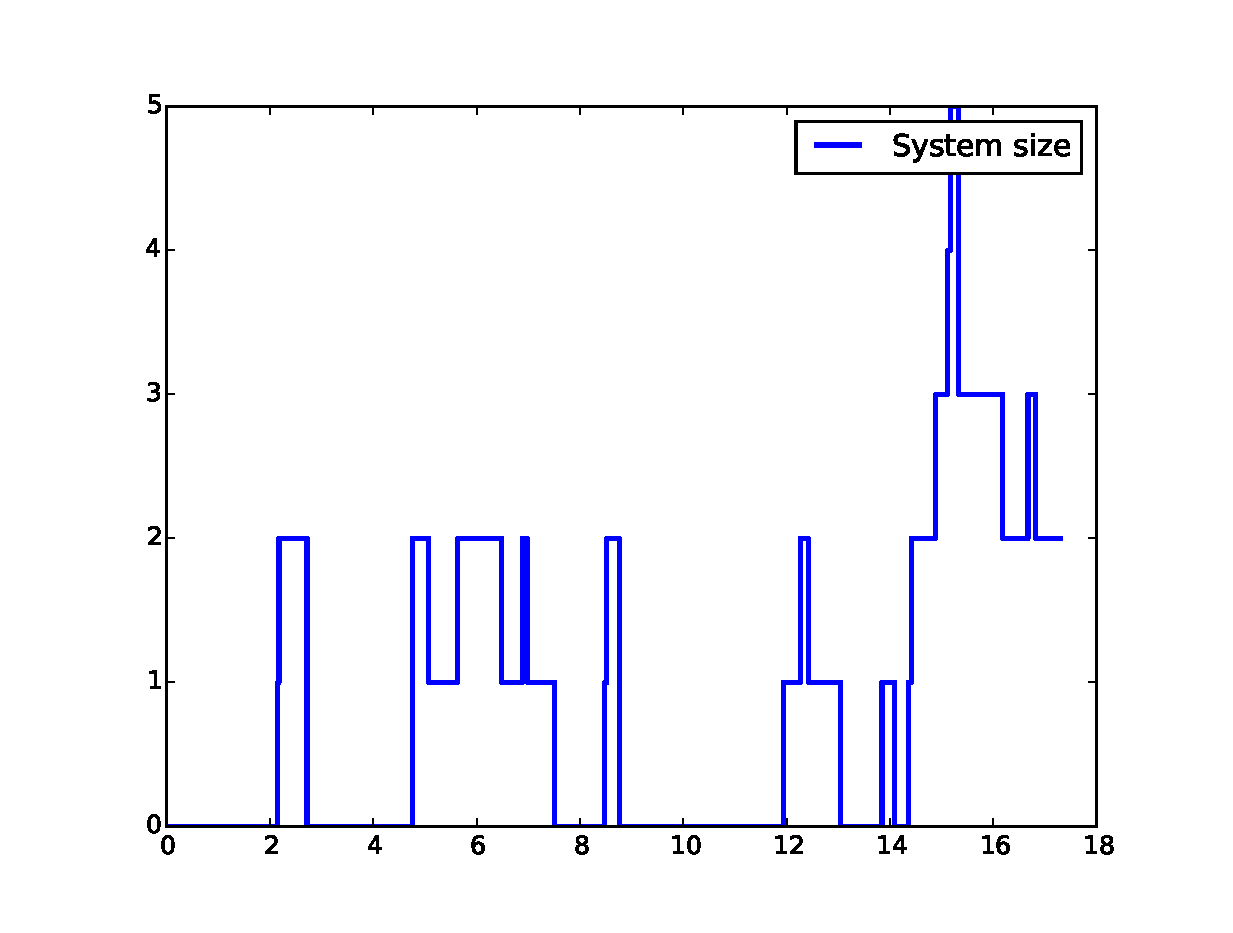
\includegraphics[width=3.3in]{md1-system-size}
\caption{M/D/1 System Size}
\label{md1-system-size}
\end{minipage}
\begin{minipage}[t]{0.5\linewidth}
\centering
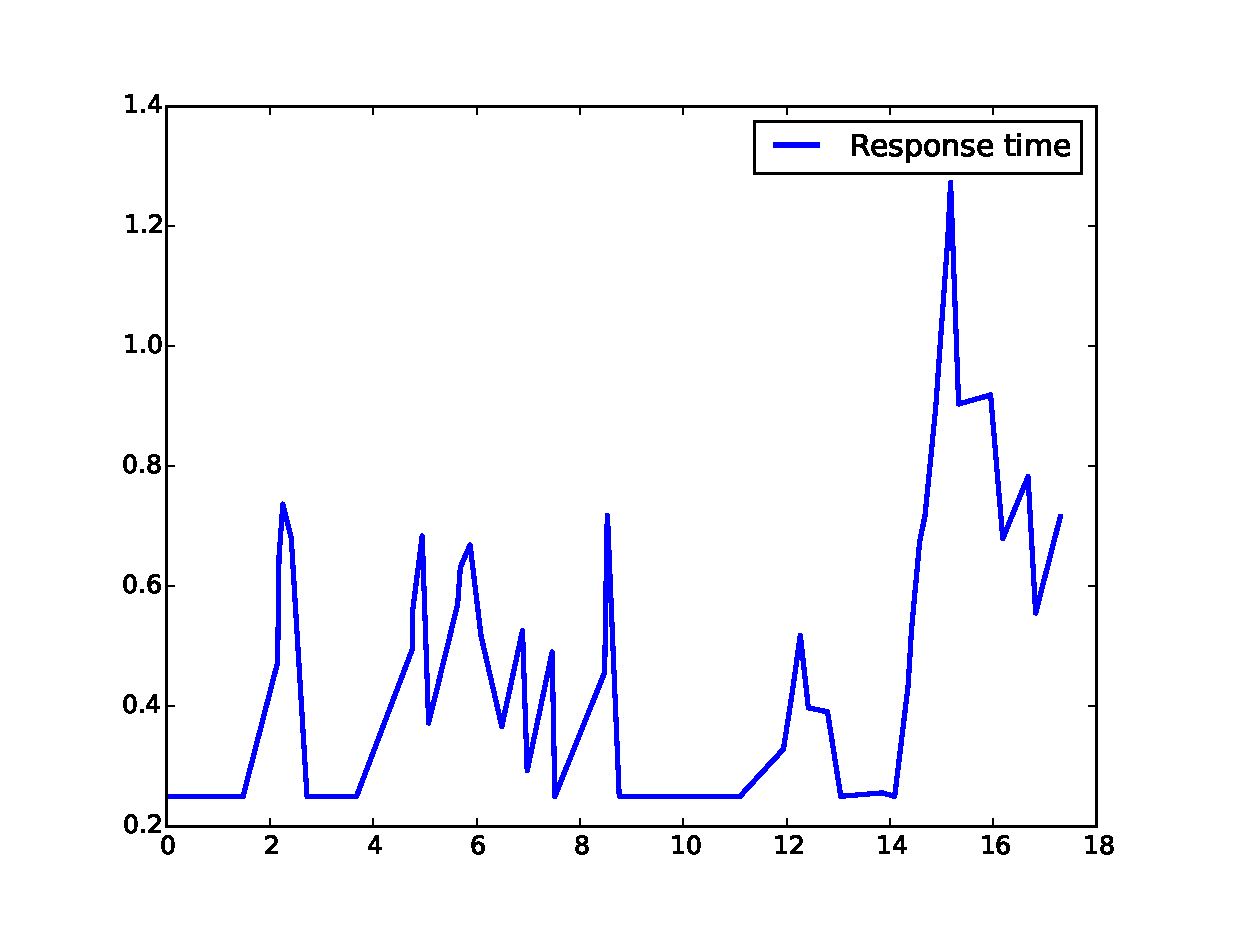
\includegraphics[width=3.3in]{md1-response-time}
\caption{M/D/1 Response Time}
\label{md1-response-time}
\end{minipage}
\end{figure}

\end{homeworkSection}

%--------------------------------------------

\begin{homeworkSection}{D/M/1}

Mean practical delay: 0.548419\\
Mean practical size : 1.197356

\begin{figure}[H]
\begin{minipage}[t]{0.5\linewidth}
\centering
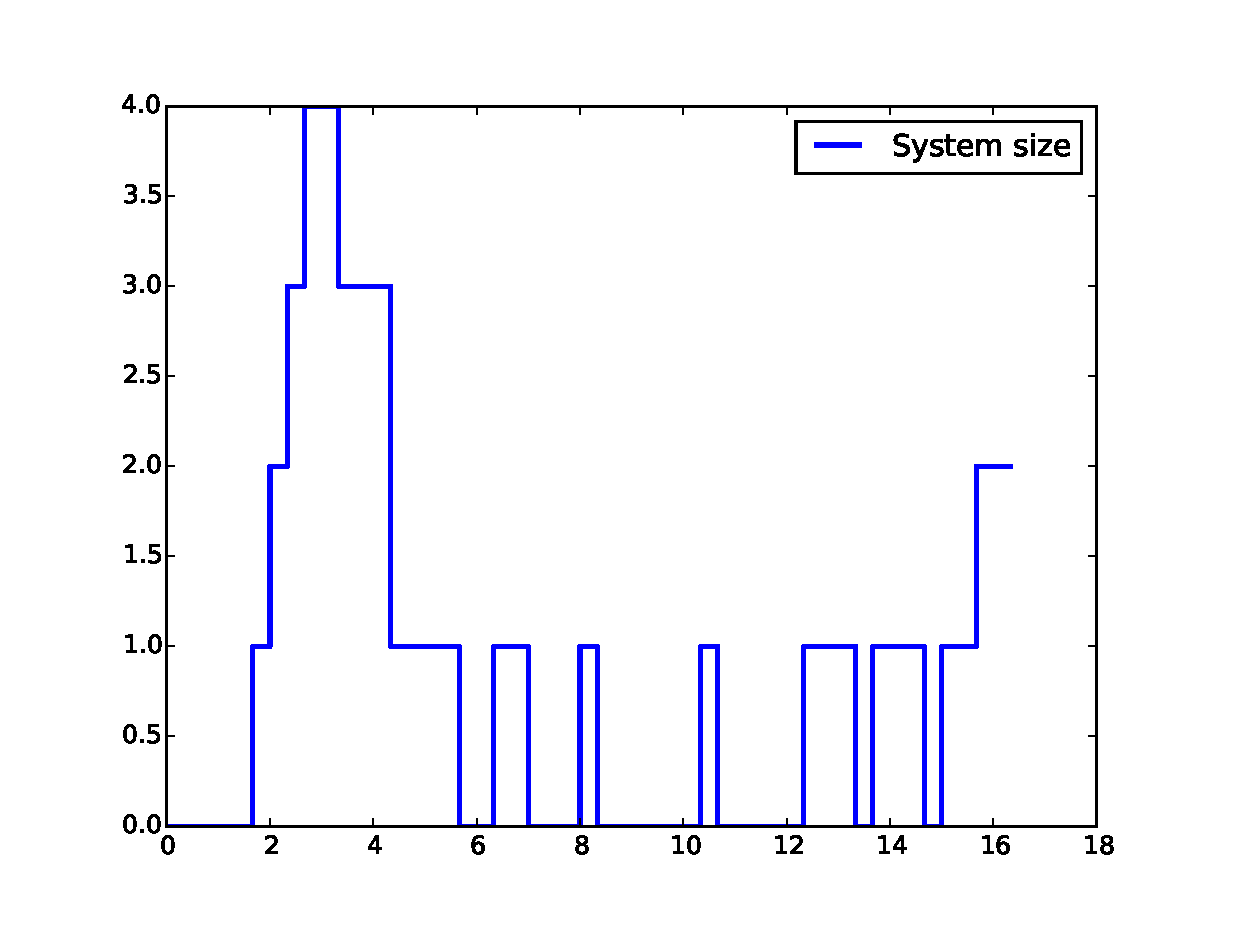
\includegraphics[width=3.3in]{dm1-system-size}
\caption{D/M/1 System Size}
\label{dm1-system-size}
\end{minipage}
\begin{minipage}[t]{0.5\linewidth}
\centering
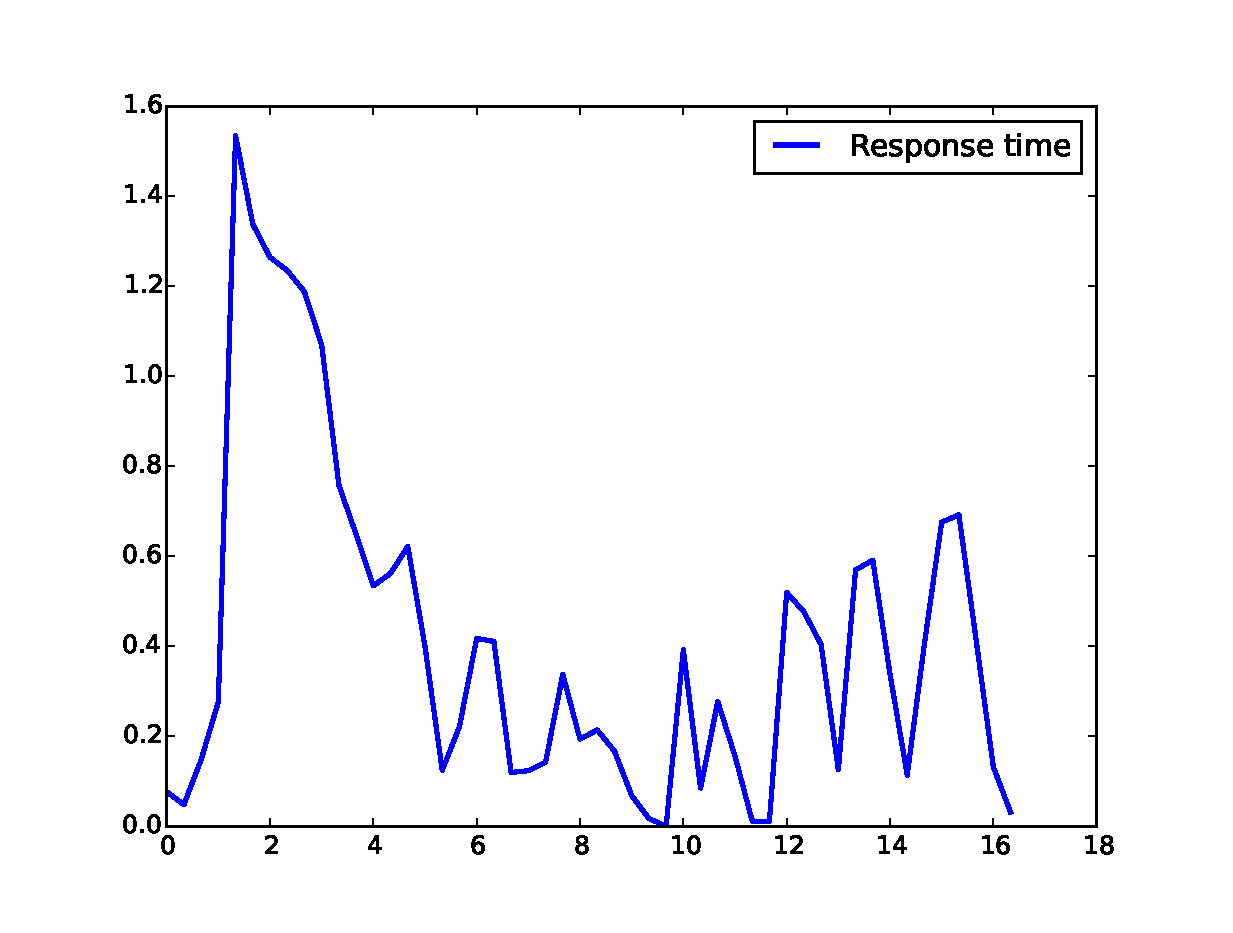
\includegraphics[width=3.3in]{dm1-response-time}
\caption{D/M/1 Response Time}
\label{dm1-response-time}
\end{minipage}
\end{figure}

\end{homeworkSection}

%--------------------------------------------

\begin{homeworkSection}{D/D/1}

Mean practical delay: 0.250000\\
Mean practical size : 0.000000

\begin{figure}[H]
\begin{minipage}[t]{0.5\linewidth}
\centering
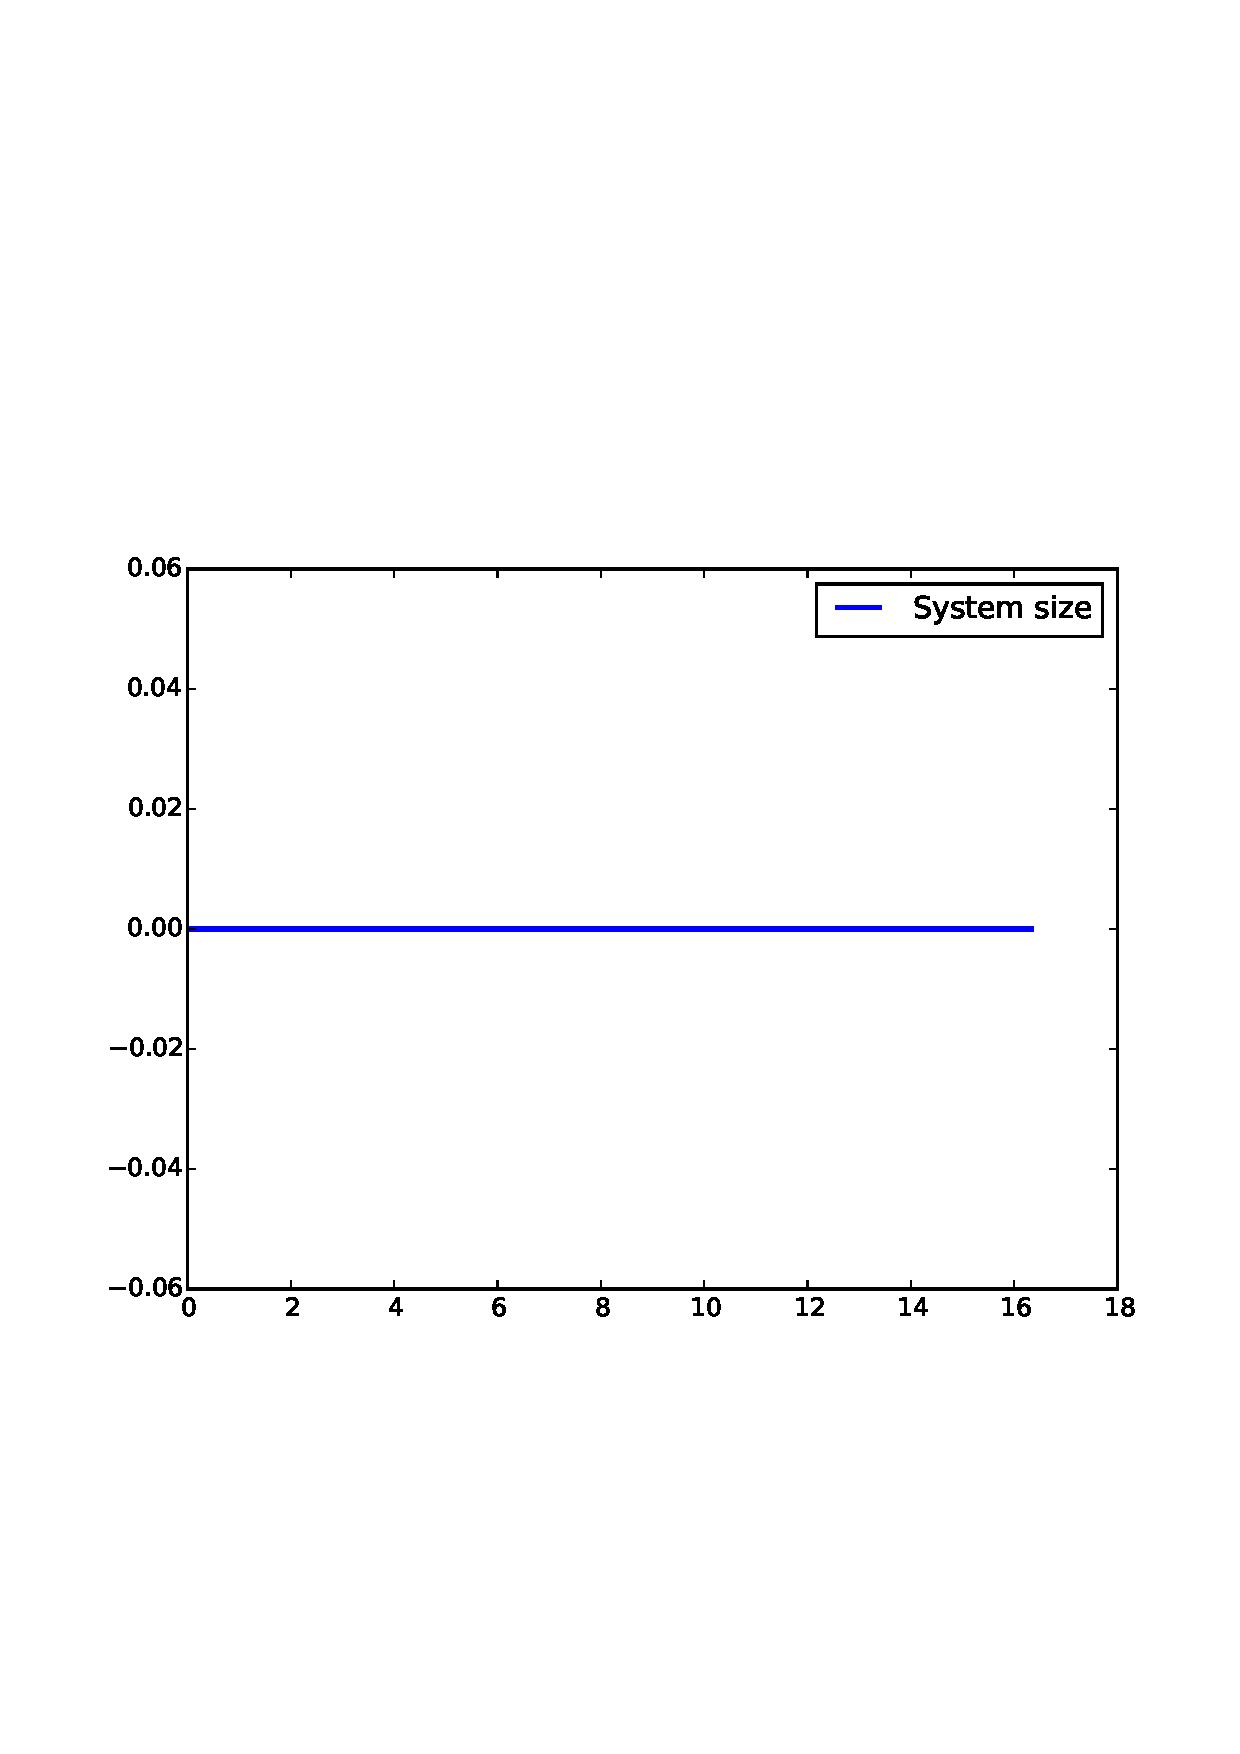
\includegraphics[width=3.3in]{dd1-system-size}
\caption{D/D/1 System Size}
\label{dd1-system-size}
\end{minipage}
\begin{minipage}[t]{0.5\linewidth}
\centering
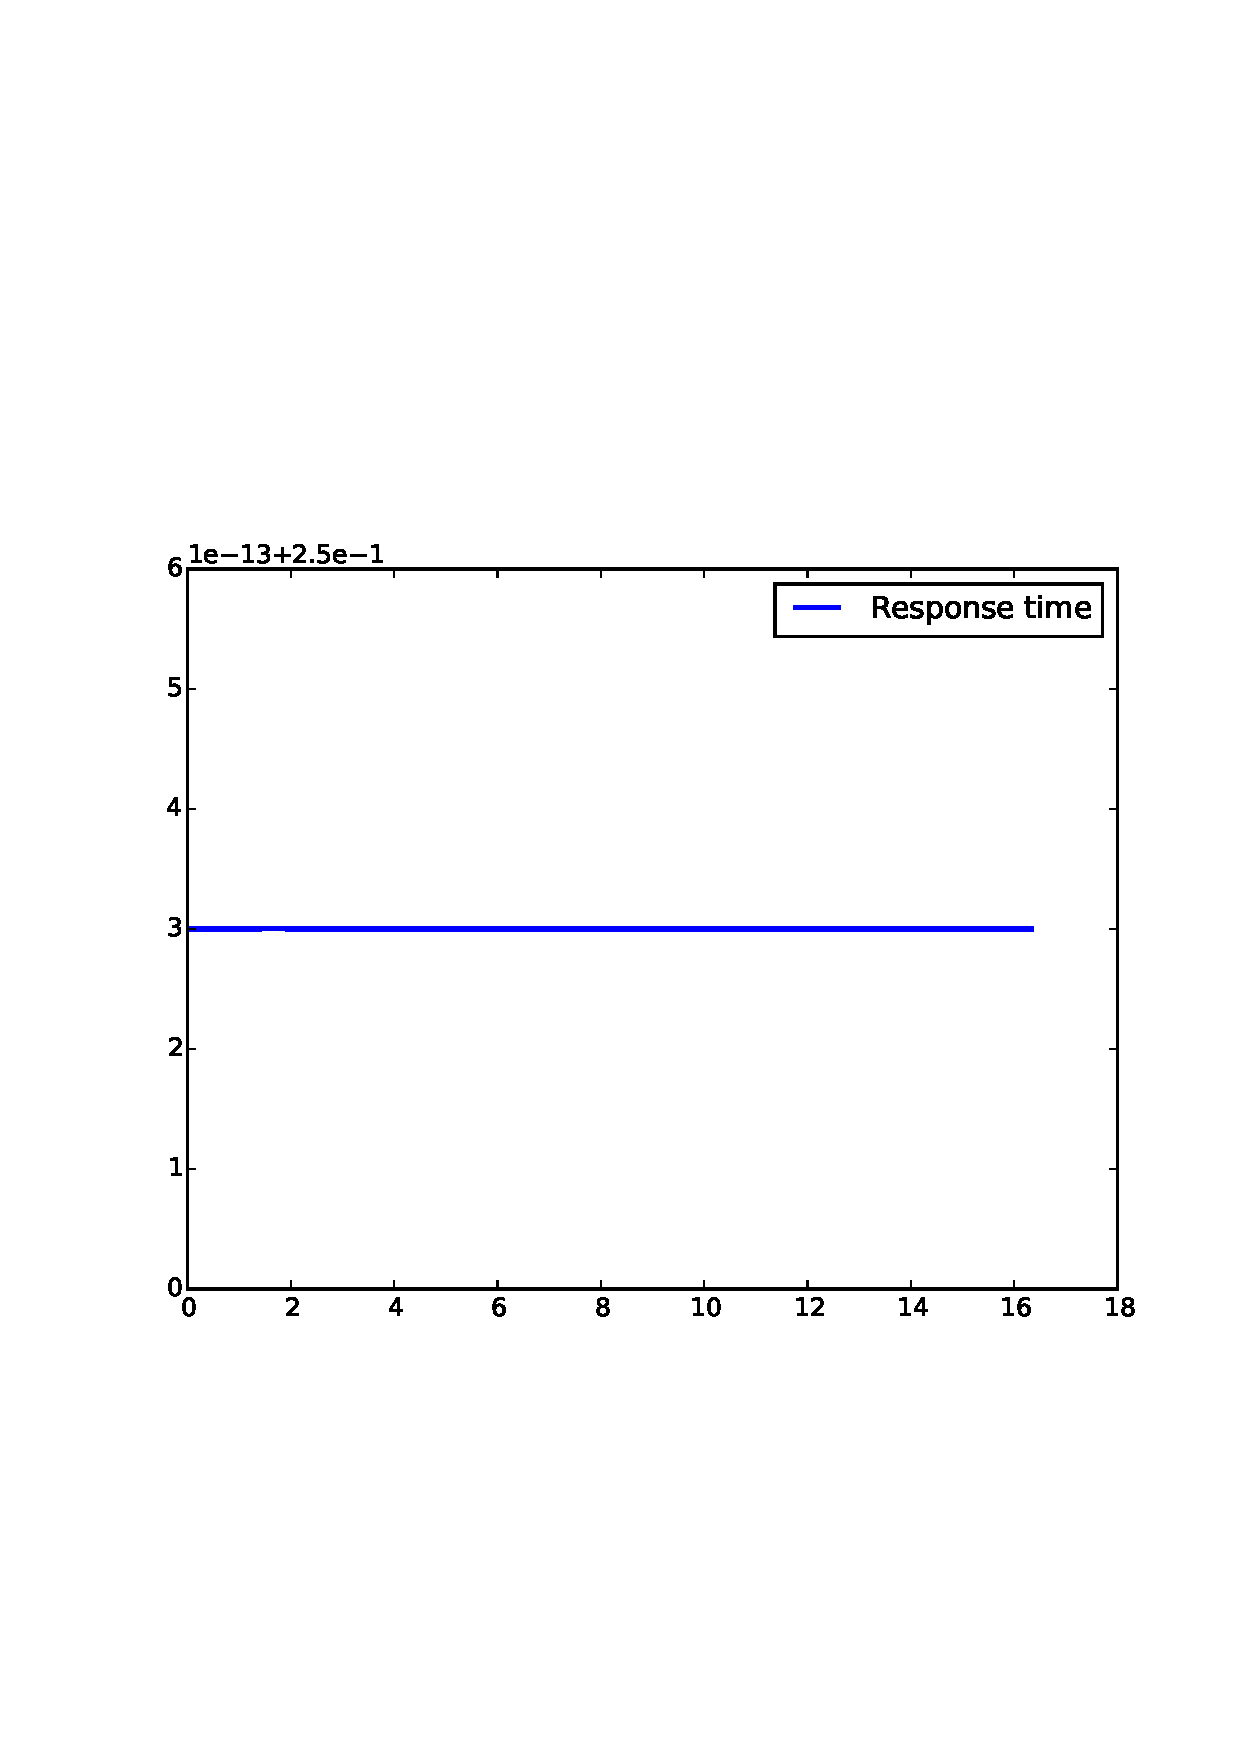
\includegraphics[width=3.3in]{dd1-response-time}
\caption{D/D/1 Response Time}
\label{dd1-response-time}
\end{minipage}
\end{figure}

\end{homeworkSection}

%--------------------------------------------

\end{homeworkProblem}

%--------------------------------------------

\begin{homeworkProblem}{Question 1.6}
Provide a working copy of the programs you have written in Step 1.2 according to the guidelines for full credit.\\

\begin{tabular}{c c}
M/M/1 &\texttt{section1/mm1.py}\\
M/D/1 &\texttt{section1/md1.py}\\
D/M/1 &\texttt{section1/dm1.py}\\
D/D/1 &\texttt{section1/dd1.py}
\end{tabular}
\end{homeworkProblem}

%----------------------------------------------------------------------------------------
%	Section 2
%----------------------------------------------------------------------------------------

\begin{homeworkProblem}{Question 2.1}
Provide a working copy of the program you write in this step according to the guidelines for full credit.\\

Mean practical delay: 1.067071\\
Mean practical size : 5.327433\\

Mean theoretical delay: 1.090909\\
Mean theoretical size : 5.454545\\

Program: \texttt{section2/mmc.py}
\end{homeworkProblem}

%--------------------------------------------

\begin{homeworkProblem}{Bonus Question}
Experiment with other queue types, e.g. M/D/2, D/M/2, D/D/2. Especially, investigate queue stability for various parameters and briefly interpret your observations.\\

$m$ the number of servers\\
$\lambda$ arrival rate\\
$\mu$ service rate per server\\

$\lambda \le m \mu$ is the stability requirement. When $\lambda > m \mu$, the queuing system becomes unstable.\\

\begin{tabular}{c c}
M/D/2 &\texttt{section2/mdc.py}\\
D/M/2 &\texttt{section2/dmc.py}\\
D/D/2 &\texttt{section2/ddc.py}
\end{tabular}
\end{homeworkProblem}

%----------------------------------------------------------------------------------------
%	Section 3
%----------------------------------------------------------------------------------------

\begin{homeworkProblem}{Question 3.1}
Calculate the theoretical expected system size and the expected time spent in system for each case above (in Python or Matlab) using standard formulas.

\begin{homeworkSection}{Case 1}
Mean theoretical delay: 1.000000\\
Mean theoretical size : 5.000000
\end{homeworkSection}

\begin{homeworkSection}{Case 2}
Mean theoretical delay: 2.000000\\
Mean theoretical size : 10.000000
\end{homeworkSection}

\begin{homeworkSection}{Case 3}
Mean theoretical delay: 1.090909\\
Mean theoretical size : 5.454545
\end{homeworkSection}
\end{homeworkProblem}

%--------------------------------------------

\begin{homeworkProblem}{Question 3.2}
You have already simulated two of the three cases above. Simulate the third case and provide your working program according to the guidelines.\\

Program: \texttt{section3/Q31.py}
\end{homeworkProblem}

%--------------------------------------------

\begin{homeworkProblem}{Question 3.3}
Calculate the performance of each option based on your simulations and check your results against theoretical values.

\begin{homeworkSection}{Case 1}
Mean practical delay: 1.039124 $\approx$ 1\\
Mean practical size : 5.186733 $\approx$ 5
\end{homeworkSection}

\begin{homeworkSection}{Case 2}
Q0 mean practical delay: 2.116894\\
Q0 mean practical size : 5.257232\\
Q1 mean practical delay: 1.882052\\
Q1 mean practical size : 4.686604\\
Combined mean practical delay: 1.999473 $\approx$ 2\\
Combined mean practical size : 9.943836 $\approx$ 10
\end{homeworkSection}

\begin{homeworkSection}{Case 3}
Mean practical delay: 1.067071 $\approx$ 1.090909\\
Mean practical size : 5.327433 $\approx$ 5.454545\\
\end{homeworkSection}

Simulation results are similar to theoretical values.

\end{homeworkProblem}

%--------------------------------------------

\begin{homeworkProblem}{Question 3.4}
Which of the three options above would you choose? Why? Discuss briefly based on the simulation and theoretical analysis you have conducted.\\

Time spent in option 1 and option 3 is much shorter than in option 2. The goal is to minimize the time, so option 2 will not be adopted. Option 1 and option 3 have relatively equal waiting time, however, option 3 consisting of 3 routers is more complicated than option 1. To conclude, option 1 is the best solution.
\end{homeworkProblem}

%----------------------------------------------------------------------------------------
%	Appendix
%----------------------------------------------------------------------------------------

\newpage
\begin{homeworkProblem}{Appendix}

\begin{homeworkSection}{\texttt{section1/mm1.py}}
\lstinputlisting{mm1.py}
\end{homeworkSection}

\newpage
\begin{homeworkSection}{\texttt{section1/md1.py}}
\lstinputlisting{md1.py}
\end{homeworkSection}

\newpage
\begin{homeworkSection}{\texttt{section1/dm1.py}}
\lstinputlisting{dm1.py}
\end{homeworkSection}

\newpage
\begin{homeworkSection}{\texttt{section1/dd1.py}}
\lstinputlisting{dd1.py}
\end{homeworkSection}

%--------------------------------------------

\begin{homeworkSection}{\texttt{section2/mmc.py}}
\lstinputlisting{mmc.py}
\end{homeworkSection}

\newpage
\begin{homeworkSection}{\texttt{section2/mdc.py}}
\lstinputlisting{mdc.py}
\end{homeworkSection}

\newpage
\begin{homeworkSection}{\texttt{section2/dmc.py}}
\lstinputlisting{dmc.py}
\end{homeworkSection}

\newpage
\begin{homeworkSection}{\texttt{section2/ddc.py}}
\lstinputlisting{ddc.py}
\end{homeworkSection}

%--------------------------------------------

\newpage
\begin{homeworkSection}{\texttt{section3/Q31.py}}
\lstinputlisting{Q31.py}
\end{homeworkSection}

\newpage
\begin{homeworkSection}{\texttt{section3/mm1p.py}}
\lstinputlisting{mm1p.py}
\end{homeworkSection}

%--------------------------------------------

\end{homeworkProblem}

%----------------------------------------------------------------------------------------

\end{document}
